%% implmentation, the messy part

\section{Implementation} \label{chapter:implement}

\todo{big change - need to change a lot of this}

Algorithm is implemented in Python using PyBullet simulation. The program keeps the simulation and the logic completely separated. 
This way the simulation keeps the realism of operating within the real environment. Thus the program consists of three main part: simulation, agent and supervisor. 
Each module is run in separate thread, mimicking the ROS nodes.
Modules communicate through the bus,  using services and broadcasting.  \\
Simulation module generate the environment and control physics. 
Supervisor module has the knowledge about the simulation an the robot. It knows absolute position of the robot in the room as well as currently executed skill.\\
Agent module has implementations of operating logic, abstracting symbols, updating predicates, and low-level skills. \\
This chapter provides an overview of the system architecture and the methods employed in the implementation. The full source code repository is available online \parencite{skorupowska_symbols}.

\subsection{Environment}
A robot is a simplified version of e-Puck 2 (Figure \ref{fig:sim:robot}). It resembles its shape and have the same set of sensors and actuators. 
The only actuators are two differential wheels, which makes the robot to move non-holonomically. The sensors are: 8 LIDARs with range from 0 to 10 cm and a RGB camera with matrix of \(120 \times 160\) pixels.

\begin{figure}[htbp]
    \centering
    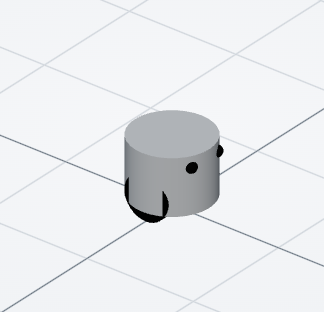
\includegraphics[width=0.8\textwidth, height=0.85\textheight, keepaspectratio]{pictures/robot_perspective.png}
    \caption{Simplified model of an e-Puck 2 as cylinder body with differential wheels. Eyes added purely for aesthetics.} 
    \label{fig:sim:robot}
\end{figure}

The arena (Figure \ref{fig:sim:arena}) for the task consist of two rooms separated by the wall. Each room has different coloured floor so the robot is able to different between them using only its sensors. 
In the separating wall there is a contrasting door. The door swings open on the push of the robot. 
Robot's task originate in orange room, then in second room, the blue one, there is contrasting post, which robot is supposed to reach.

\begin{figure}[htbp]
    \centering
    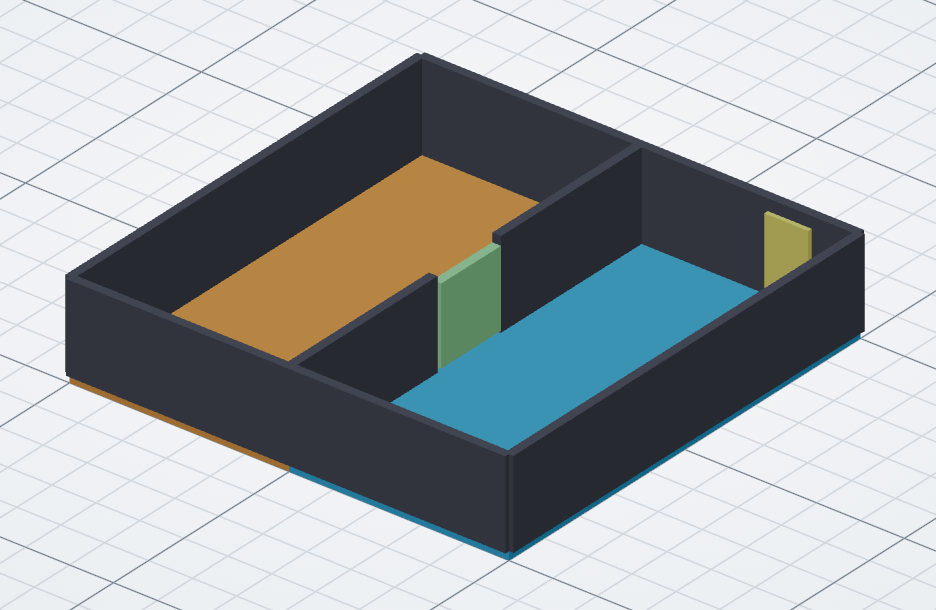
\includegraphics[width=0.8\textwidth, height=0.85\textheight, keepaspectratio]{pictures/arena_perspective.png}
    \caption{Model of an arena used in the simulation. Two rooms separated by a wall with the door.} 
    \label{fig:sim:arena}
\end{figure}

\subsection{Supervisor}
Next module updates the data for all the debugging figures and answers robot's questions through the bus. This is the implementation of supervision within the learning. 
The supervisor has knowledge beyond robot's perception and can modulate both the environment and robot. 
The main task of a supervisor in the learning process is checking if a skill was executed successfully, Each skill has some conditions of success and failure. 
This is similar to what is being learned, but the difference is that those are formulated in terms of the outsider. The outsider can have different sensors or simply different point of reference. 
For example, the supervisor knows in which room the robot is, the robot does not. The skill 'start' can be executed anywhere, has no precondition, but is finished successfully only if the robot is in the orange room.
Supervisor checks this condition and returns to the agent if it succeed.

\subsection{Agent}
This module consist of the main logic loop, the networks for predicates and transitions, and low-level skills. 

\subsubsection*{Predicates} 
Predicates are represented by Supervised Growing Neural Gas. These are implementation of basic GNG \textcite{fritzke1994gng} with added behaviour for negative points. 
The original algorithm was for unsupervised learning, and mapped space from collected points. Since the execution can be successful or not, 
I added a reverse logic for negative points, symmetrical to treating positive ones. If a point considered is positive, the neural gas points are pulled to it. 
If it is negative, they are pushed away. 
\todo{add parameters with explanation for them}

\subsubsection*{Transition graph} 
The transition graph is represented by a standard directed graph. It plays no role in the learning process. This graph is used for generating PDDL files.  
The transitions are collected from the overlapping points of effects and preconditions and generated after each update to either of them.  

\subsubsection*{PDDL files} 
PDDL files are generated by simple, structural code. Each time the predicates are updated, the new problem and domain files are generated. 
The domain file (Listing \ref{lst:pddl:domain}) defines the world for an agent. What can be seen (predicates) and what can be done (actions). In this domain there are as many actions as skills, and for each skill two types of predicates: can-run-skill and executed-skill. This way we cover both starting conditions for a skill and its effect.
The problem file (Listing \ref{lst:pddl:problem}) specify the domain and the predicates that are fulfilled at the beginning and the predicates that need to be fulfilled at the end.
   
\begin{lstlisting}[caption={Problem definition in PDDL}, label={lst:pddl:problem}]
(define (problem plan_problem)
  (:domain robot_domain)
  (:init
    (can_run_Start)
  )
  (:goal
    (executed_Finish)
  )
)
\end{lstlisting}
\begin{lstlisting}[caption={Domain definition in PDDL}, label={lst:pddl:domain}]
(define (domain robot_domain)
  (:requirements :strips)
  (:predicates
    (can_run_Open_the_Door)
    (executed_Open_the_Door)
    (can_run_Start)
    (executed_Start)
    (can_run_Finish)
    (executed_Finish)
    (can_run_Go_to_the_Goal)
    (executed_Go_to_the_Goal)
    (can_run_Go_to_the_Door)
    (executed_Go_to_the_Door)
    (can_run_Find_the_Door)
    (executed_Find_the_Door)
    (can_run_Find_the_Goal)
    (executed_Find_the_Goal)
  )

  (:action Open_the_Door
    :parameters ()
    :precondition (can_run_Open_the_Door)
    :effect (and (executed_Open_the_Door) (can_run_Find_the_Door) (can_run_Find_the_Goal) (not (can_run_Open_the_Door)))
  )

  (:action Start
    :parameters ()
    :precondition (can_run_Start)
    :effect (and (executed_Start) (can_run_Find_the_Door) (not (can_run_Start)))
  )

  (:action Finish
    :parameters ()
    :precondition (can_run_Finish)
    :effect (and (executed_Finish) (not (can_run_Finish)))
  )

  (:action Go_to_the_Goal
    :parameters ()
    :precondition (can_run_Go_to_the_Goal)
    :effect (and (executed_Go_to_the_Goal) (can_run_Finish) (can_run_Find_the_Door) (can_run_Find_the_Goal) (not (can_run_Go_to_the_Goal)))
  )

  (:action Go_to_the_Door
    :parameters ()
    :precondition (can_run_Go_to_the_Door)
    :effect (and (executed_Go_to_the_Door) (can_run_Open_the_Door) (can_run_Find_the_Door) (not (can_run_Go_to_the_Door)))
  )

  (:action Find_the_Door
    :parameters ()
    :precondition (can_run_Find_the_Door)
    :effect (and (executed_Find_the_Door) (can_run_Go_to_the_Door) (not (can_run_Find_the_Door)))
  )

  (:action Find_the_Goal
    :parameters ()
    :precondition (can_run_Find_the_Goal)
    :effect (and (executed_Find_the_Goal) (can_run_Go_to_the_Goal) (not (can_run_Find_the_Goal)))
  )
)
\end{lstlisting}

\subsubsection*{Visual Preprocessing}

\subsubsection*{Low-level Skills}